\documentclass{standalone}
\usepackage{tikz}
\usetikzlibrary{arrows}
\usetikzlibrary{arrows.meta}

\begin{document}
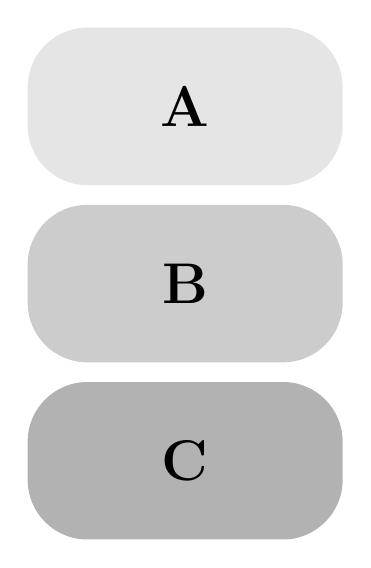
\begin{tikzpicture}

\fill[gray!20,rounded corners=5ex] (-2,-2) rectangle (2,0);
\fill[gray!40,rounded corners=5ex] (-2,-4.25) rectangle (2,-2.25);
\fill[gray!60,rounded corners=5ex] (-2,-6.5) rectangle (2,-4.5);

\draw (0,-1) node{\huge{\textbf{A}}} ; 
\draw (0,-3.25) node{\huge{\textbf{B}}} ; 
\draw (0,-5.5) node{\huge{\textbf{C}}} ; 


\end{tikzpicture}
\end{document}
